\documentclass[a4paper,11pt]{article}

\usepackage[utf8]{inputenc}
\usepackage[T1]{fontenc}
\usepackage{babel}
\usepackage[top=2.5cm, bottom=2.5cm, left=2.5cm, right=2.5cm]{geometry}
\usepackage{xcolor}
\usepackage{hyperref}
\usepackage{titlesec}
\usepackage{enumitem}
\usepackage{mdframed}
\usepackage{fancyhdr}
\usepackage{graphicx}

% Couleurs
\definecolor{violetuniv}{RGB}{100, 50, 150}
\definecolor{rougetitre}{RGB}{200, 50, 50}
\definecolor{borduregrise}{RGB}{180, 180, 180}

% Liens hypertexte
\hypersetup{
    colorlinks=true,
    linkcolor=violetuniv,
    urlcolor=violetuniv,
}

% Style des titres de section
\titleformat{\section}{\large\bfseries}{}{0em}{}
\titleformat{\subsection}{\normalsize\bfseries}{}{0em}{}

% En-tête
\pagestyle{fancy}
\fancyhf{}
\renewcommand{\headrulewidth}{0.4pt}
\fancyhead[L]{\small\textcolor{violetuniv}{Conception Web -- Semestre 2}}
\fancyfoot[C]{\thepage}

% Environnement "À faire"
\newmdenv[
    linecolor=borduregrise,
    backgroundcolor=white,
    linewidth=1pt,
    leftmargin=0pt,
    rightmargin=0pt,
    innerleftmargin=10pt,
    innerrightmargin=10pt,
    innertopmargin=8pt,
    innerbottommargin=8pt,
]{afaire}

\begin{document}

% ============================================================
% PAGE DE PRÉSENTATION
% ============================================================
\thispagestyle{empty}
\vspace*{3cm}

\begin{center}
    {\small\textcolor{violetuniv}{Université d'Avignon -- CERI}}\\[0.5cm]
    {\small\textcolor{violetuniv}{Licence Informatique -- Semestre 2}}\\[2cm]

    {\rule{\linewidth}{0.5pt}}\\[0.4cm]
    {\LARGE\bfseries Conception Web}\\[0.3cm]
    {\large TP1 -- Bases de HTML, tableaux et liens}\\[0.4cm]
    {\rule{\linewidth}{0.5pt}}\\[2cm]

    {\large Module : S-E06-0158}\\[0.5cm]
    {\large Année universitaire 2025--2026}\\[3cm]

    \begin{tabular}{ll}
        \textbf{Enseignant :} & Fabrice Lefèvre \\
        \textbf{Niveau :}     & Licence 1 Informatique \\
        \textbf{Semestre :}   & Semestre 2 \\
    \end{tabular}
\end{center}

\vfill

\begin{center}
    \textcolor{borduregrise}{\rule{\linewidth}{0.3pt}}\\[0.3cm]
    {\small\textit{Ce document regroupe les sujets des TP 1.1 et 1.2 du module Conception Web.}}
\end{center}

% ============================================================
\newpage
\fancyhead[R]{\small TP 1.1 -- Mise en forme de texte et tableaux}

{\Large\bfseries TP 1.1 -- Mise en forme de texte et tableaux}

\bigskip

\section{Mise en forme de texte et tableaux}

L'ensemble des exemples demandés ci-dessous doivent être regrouper dans un seul fichier HTML, pour passer en revue les balises principales de mise en forme du texte.

\textcolor{rougetitre}{\textbf{Attention}} : pour ce TP il n'est pas demandé d'utiliser CSS. Les ``anciennes'' balises de mise en forme de texte pourront être utilisées et on observera que le validateur (voir TP0) indique que ces choix sont obsolètes. Toutefois si votre documentation de référence vous indique directement du CSS (en général en passant par l'attribut \texttt{style}) alors n'hésitez pas à l'utiliser.

\subsection{A faire :}

\begin{afaire}
\textbf{Mise en forme et structuration d'un texte}

\begin{itemize}
    \item Mettre en forme l'article disponible dans le fichier \texttt{tp1.txt} en ajoutant le squelette de base HTML.
    \item Utiliser les balises de titres, de paragraphes et de mise en forme (\texttt{em}, \texttt{strong}, \texttt{u}, \texttt{mark}\ldots) pour structurer le contenu et mettre en évidence les éléments importants.
\end{itemize}

\textbf{Travail sur les citations}

\begin{itemize}
    \item Insérer au moins deux citations en utilisant les balises \texttt{<q>} et \texttt{<blockquote>}.
    \item Ajouter un court texte explicatif sur la différence d'affichage entre ces deux balises.
\end{itemize}

\textbf{Expérimentation de balises diverses}

À la suite du texte de \texttt{tp1.txt}, ajouter :

\begin{itemize}
    \item Un \textbf{extrait de code C++} mis en forme avec \texttt{<pre>} et \texttt{<code>}, tout en préservant l'indentation et en affichant la police en bleu (via l'attribut \texttt{style} directement dans la balise \texttt{<code>}).
    \item Un \textbf{poème ou un dialogue de théâtre} mis en forme avec \texttt{<pre>} pour respecter la mise en page, et entouré d'un \texttt{<blockquote>}.
    \item Un paragraphe mathématique contenant des variables mises en valeur avec \texttt{<var>} et un exposant ``$^3$'' affiché grâce à une entité caractère.
    \item Insérer une ligne de séparation (\texttt{<hr>}) de longueur 70\% entre chaque partie du nouveau fichier \texttt{tp1.txt}.
\end{itemize}

Exemple de phrase à insérer :

\textit{``L'équation \textbf{y = mx$^3$ + b} utilise les variables \texttt{<var>y</var>} et \texttt{<var>x</var>}.''}

\textbf{Utilisation des tableaux simples}

On cherche à reproduire le petit tableau suivant
(voir annexe \ref{annexe:tab1}, page \pageref{annexe:tab1}) :

\begin{itemize}
    \item Ajouter le tableau précédent dans le document créé au début de ce TP.
\end{itemize}

On pourra l'améliorer en utilisant l'entité caractères de l'euro \texteuro, à la place du ``E''. Et, attention, la deuxième ligne contient une seule cellule pour les 2 colonnes.

\textbf{Tableaux complexes}

L'objectif de ces exercices est de reconstituer les tableaux décrits ci-après en utilisant :

\begin{enumerate}
    \item les balises
    \begin{itemize}
        \item \texttt{<thead>}
        \item \texttt{<tbody>}
        \item \texttt{<tfoot>}
        \item \texttt{<colgroup>}
        \item \texttt{<th>}
        \item \texttt{<td>}
        \item \texttt{<caption>}
    \end{itemize}
    \item les attributs
    \begin{itemize}
        \item \texttt{width}
        \item \texttt{align}
        \item \texttt{valign}
        \item \texttt{border}
        \item \texttt{colspan}
        \item \texttt{rowspan}
        \item \texttt{span}
        \item \texttt{rules}
    \end{itemize}
\end{enumerate}

\textcolor{rougetitre}{\textbf{Attention}} : pour l'instant, pour simplifier, essayer d'utiliser les attributs directement, donc pas de CSS (qui sera vu dès le TP suivant). Même s'ils ne sont plus supportés par HTML5, ils devraient s'afficher correctement dans votre navigateur.

\textcolor{rougetitre}{\textbf{Attention 2}} : du coup peut-être que \textbf{certains ne sont plus documentés sur w3schools} (les chercher ailleurs dans ce cas) : cela vous illustre bien le problème de travailler de façon constante sur la bonne version du langage (ce petit exercice est le seul pour lequel on vous fera varier de cette position).

Le tableau ressemblera \textbf{à quelques détails près} à cela
(voir annexe \ref{annexe:tab2}, page \pageref{annexe:tab2}) :

\begin{enumerate}
    \item Déclarer un tableau de largeur 75\% de la largeur de la fenêtre, aligné au centre, avec une bordure de 3
    \item Déclarer un entête au tableau (balise \texttt{<thead>}), constitué d'une ligne de trois colonnes de type header, avec comme contenu ``Colonne 1''\ldots
    \item Déclarer un \texttt{<tbody>}
    \item Déclarer une première ligne constituée de trois cellules simples. Le contenu des cellules sera le même pour toutes ``Contenu nxm'' avec n le numéro de la ligne et m de la colonne.
    \item Déclarer la deuxième ligne constituée de deux colonnes assemblées, et d'une troisième colonne
    \item Aligner le texte au centre dans la première cellule de la ligne
    \item Déclarer une troisième ``ligne'' constituée de deux cellules simples, et d'une cellule assemblant deux lignes
    \item Aligner le texte en bas dans la dernière colonne
    \item Déclarer une quatrième ligne constituée de deux cellules simples (expérimenter ce qui se passe en déclarant une cellule de moins, ou une cellule de plus ; interpréter le résultat)
    \item Déclarer une cinquième ligne constituée d'une cellule simple et d'une cellule regroupant deux colonnes et deux lignes
    \item Aligner le texte à droite et en haut dans la dernière cellule
    \item Compléter le tableau par une dernière ligne. Combien faut-il de cellules ?
\end{enumerate}

\textcolor{rougetitre}{\textbf{Compléments}} : Copiez le code du tableau élaboré ci-dessus, placez-le à la suite et essayez les effets des autres balises et attributs disponibles.

\textbf{Tableaux complexes 2}

Dans les mêmes conditions que l'exercice précédent, reproduire le tableau suivant
(voir annexe \ref{annexe:tab3}, page \pageref{annexe:tab3}).

(Placez-le dans le même fichier, à la suite du code de l'exercice précédent.)

\textcolor{rougetitre}{\textbf{Attention}} : ce tableau contient des cellules SANS BORDURES (ce qui donne l'impression d'une seule cellule multi-ligne). Pour reproduire cet effet, il faut faire les bons regroupements de cellules de base et ensuite demander à n'afficher que les bordures (``rules'') entre GROUPES (groupe de colonnes définis avec \texttt{colgroup}, groupes de lignes définis avec \texttt{tbody}, \texttt{thead} ou \texttt{tfoot}).

\end{afaire}

\vspace{1em}
\noindent\textcopyright{} Sujet proposé par Fabrice Lefèvre, 2026

\vspace{0.5em}
\noindent\textit{Last modified: Wednesday, 18 March 2026, 8:41 AM}

% ============================================================
\newpage
\fancyhead[R]{\small TP 1.2 -- Liens hypertextes et listes}

{\Large\bfseries TP 1.2 -- Liens hypertextes et listes}

\bigskip

\section{Liens hypertextes et listes}

\subsection{1. Liens relatifs et listes}

Afin de simuler l'organisation des pages web au sein d'un site, nous allons créer des fichiers ne contenant que des liens les uns vers les autres. Lorsqu'ils désignent des documents présents sur le même serveur on parle de liens \textit{relatifs}. En pratique il n'est plus impératif de donner une URL complète dans ce cas, c'est à dire sous la forme ``service://serveur/repertoires/fichier''. Le service et le serveur sont connus par défaut on ne précise donc que le chemin d'accès du fichier sur le serveur. Mais attention pour cela on indique ce chemin à partir du répertoire qui contient notre page d'appel (ie le fichier qui contient le lien).

\textbf{Rappels} sur l'écriture des URL relatives -- 4 cas pour un lien de type \texttt{<a href="monfichier">Ici pour afficher mon fichier</a>} :

\begin{enumerate}
    \item Ressource située dans le \textbf{même répertoire} que la page d'appel (ie le fichier qui contient le lien) : la valeur prise par l'attribut \texttt{href} est simplement le nom du fichier, par exemple \texttt{href="index.html"}.
    \item Ressource située dans un \textbf{sous-répertoire} du répertoire contenant la page d'appel : il faut citer la suite des sous-répertoires pour ``descendre'' jusqu'au fichier ressource, par exemple \texttt{href="archives/2021/989374.html"}.
    \item Ressource située dans un \textbf{répertoire contenant} la page d'appel : il faut ``remonter'' successivement chaque répertoire par ``\texttt{../}''. Dans cet exemple, le répertoire visé est le supérieur hiérarchique de deuxième rang (le grand-père) : \texttt{href="../../index.html"}.
    \item Ressource située dans une \textbf{branche latérale} : il faut remonter au répertoire commun par ``\texttt{../}'' puis redescendre la bonne branche, par exemple \texttt{href="../../produits/convecteurs/rh1200x.html"}.
\end{enumerate}

\begin{afaire}
\textbf{A faire :}

\begin{itemize}
    \item Créer la structure de répertoires (dossiers) suivante dans votre espace de stockage personnel
    (voir annexe \ref{annexe:arbo}, page \pageref{annexe:arbo}).
    \item Créer ensuite \textbf{vous-même} chacun des 5 fichiers html selon le schéma précédent en les plaçant dans les dossiers correspondants.
    \begin{itemize}
        \item Chaque fichier devra contenir seulement un menu : une liste (numérotée) de liens relatifs vers tous les autres fichiers.
    \end{itemize}
    \item Vérifier à la fin qu'on peut atteindre tous les fichiers depuis n'importe lequel d'entre eux.
    \item Enfin en guise de contenu pour le fichier \texttt{exemple.html} ajouter une liste numérotée imbriquée dans une liste non numérotée imbriquée dans une liste non numérotée. Items des listes au choix (i.e. leur contenu est sans importance).
\end{itemize}
\end{afaire}

\textcolor{rougetitre}{\textbf{Important}} : il faut privilégier les liens relatifs dans les documents HTML ! En effet, lors de la création d'un site destiné à être accessible sur un seul serveur (cas général), tous les liens internes doivent être sous forme relative. Car on développe sur sa propre machine avant de transférer l'ensemble du site créé sur le serveur. Si les liens internes sont sous forme absolue (``http://nom du serveur/rep1/rep1.8/document.html''), ils ne seront plus valides après le transfert (puisque les répertoires ne seront pas forcement les mêmes sur le serveur).

\subsection{2. Ancres nommées et liens internes}

Dans ce second exercice, on va utiliser les \textit{liens internes} à une page. Dans ce cas les liens ne modifient pas la page affichée mais la partie de la page visible dans la zone d'affichage en se déplaçant vers un emplacement indiqué dans le lien. Pour cela l'URL de base peut être complétée par une ancre nommée au sein du fichier, en ajoutant un ``\#'' sous la forme \texttt{http://nom du serveur/repertoires/monfichier.html\#exercice2} par exemple. On peut donc utiliser cette capacité entre des documents différents. Et on peut la simplifier en \texttt{\#exercice2} au sein du même fichier. Il ne reste plus qu'à créer l'emplacement visé sous la forme d'une ancre nommée, qui est un lien avec un nom (attribut ``\texttt{id}'').

\begin{afaire}
\textbf{A faire :}

\begin{itemize}
    \item Sauvegarder le fichier html de ce sujet de TP (donc la page que vous avez sous les yeux actuellement) dans votre espace de stockage. Voir le TP0, si vous ne savez pas faire.
    \item Insérer une table des matières hypertexte au début du fichier : c'est à dire la liste des titres de niveau H3 présents dans le sujet avec des liens vers les titres eux-mêmes qui se trouveront plus bas dans le corps du sujet. Pour cela il faut :
    \begin{itemize}
        \item Créer une ancre nommée au niveau de chaque titre
        \item Créer un lien ``Retour au sommaire'' vers le sommaire au niveau de chaque titre (pour remonter instantanément au début de la page)
        \item Créer le sommaire en début de page : c'est à dire une liste de liens internes à la page vers les ancres nommées
    \end{itemize}
    \item Créer une ancre nommée ``HAUT DE LA PAGE''. Placer un lien vers cette ancre en bas de votre page. Cette ancre va vous permettre de revenir au début de votre page web.
    \item Au niveau de chaque titre d'exercice, insérer un nouveau lien vers le fichier qui contient la réponse.
\end{itemize}
\end{afaire}

\textcolor{rougetitre}{\textbf{Important}} : vous avez maintenant une idée pour faire des archives de rendu de TP correctes. La dernière étape devra être reproduite à partir de maintenant pour tous les rendus de TP, afin de faciliter la manipulation des rendus par vos chargés de TP et aussi de vous constituer une base d'archive facilement utilisable plus tard.

\vspace{1em}
\noindent\textcopyright{} Sujet proposé par Fabrice Lefèvre, 2026

\vspace{0.5em}
\noindent\textit{Last modified: Wednesday, 18 March 2026, 8:42 AM}

% ============================================================
% ANNEXES
% ============================================================
\newpage
\fancyhead[R]{\small Annexes}
\appendix

\section{Tableau simple Euros/Francs -- TP 1.1}
\label{annexe:tab1}

\begin{center}
    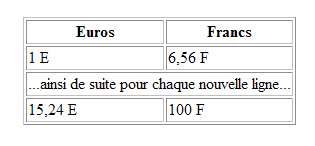
\includegraphics[width=0.45\textwidth]{TP1_1.1-tab1.png}
\end{center}

\section{Tableau complexe -- TP 1.1}
\label{annexe:tab2}

\begin{center}
    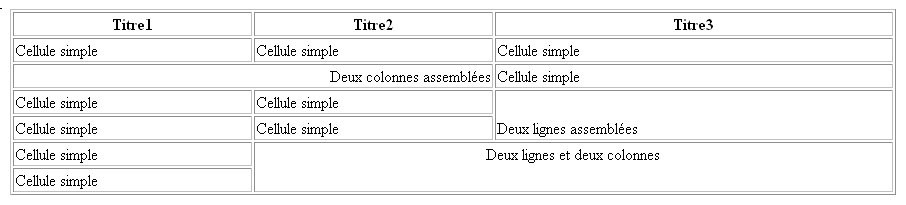
\includegraphics[width=0.95\textwidth]{TP1_1.1-tab2.jpg}
\end{center}

\section{Tableau complexe 2 (Kumquats) -- TP 1.1}
\label{annexe:tab3}

\begin{center}
    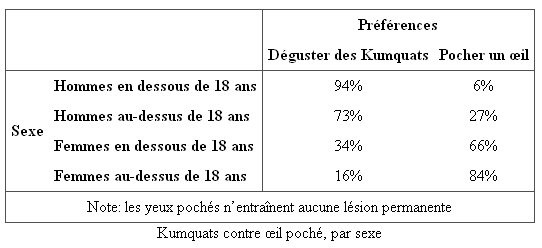
\includegraphics[width=0.75\textwidth]{TP1_1.1-tab3.jpg}
\end{center}

\section{Arborescence de répertoires -- TP 1.2}
\label{annexe:arbo}

\begin{center}
    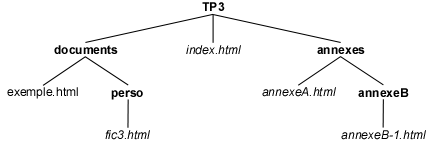
\includegraphics[width=0.6\textwidth]{TP_1.2-arbo.png}
\end{center}

\end{document}